\documentclass[10pt, conference, compsocconf]{IEEEtran}

% correct bad hyphenation here
\hyphenation{op-tical net-works semi-conduc-tor}

\usepackage[pdftex]{graphicx}

\begin{document}
%
% paper title
% can use linebreaks \\ within to get better formatting as desired
\title{Tool Demo: The MPS Language Workbench}


% author names and affiliations
% use a multiple column layout for up to two different
% affiliations

\author{\IEEEauthorblockN{Markus Voelter}
\IEEEauthorblockA{independent/itemis\\
voelter@itemis.de}
\and
\IEEEauthorblockN{Vaclav Pech}
\IEEEauthorblockA{JetBrains\\
vaclav.pech@jetbrains.com}
}

\newcommand\todo[1]{\mynote{TODO}{#1}} 
\newcommand{\fig}[1]{Fig.~\ref{#1}}
\newcommand{\sect}[1]{Section~\ref{#1}}
\newcommand{\ic}[1]{\changefont{cmtt}{m}{n}{#1}\normalfont}  % inline code
\newcommand{\lcr}[1]{\changefont{cmtt}{m}{n}{#1}\normalfont} % language

\newcommand{\pp}[1]{ \vspace{2mm}\noindent\textbf{{#1}} }


% make the title area
\maketitle


\begin{abstract}
The JetBrains MPS is a comprehensive environment for language engineering.
New languages can be defined as standalone languages or as modular extensions of
existing languages. Since MPS is a projectional editor, syntactic forms other
than text are possible, including tables or mathematical symbols. In this
session, we will \todo{}
\end{abstract}

\begin{IEEEkeywords}
language engineering, language extension, language composition
\end{IEEEkeywords}

\section{Introduction and Motivation}

\noindent
Finding and working with the right abstractions for describing a
problem or its solution is one of the central pillars of software engineering.
Once the right abstractions have been found, things can be expressed more
concisely, are easier to understand, the description can be analysed and other
artifacts can be synthesized. A language is the purest form of abstraction,
adding a suitable concrete syntax to work with the abstractions effectively. An
IDE that supports syntax coloring, code completion, error annotation and
refactoring makes working with the language and its abstractions even more
productive.

Many software systems are composed from several concerns, each of them expressed
with its own set of abstraction, possibly by different people, some of them may
not even be programmers. So, to describe a real-world system, ideally several
languages are necessary.

Looking at software engineering in this light, an environment is needed in
which language creation is easy, languages can be composed and the concrete
syntax is very flexible to encompass the needs of all the stakeholders involved
in the software system. The JetBrains MPS open source language workbench is such
as system.

\section{How MPS Works}

\noindent
MPS is a projectional editor. This means that a wide variety of syntactic forms
are supported including textual, symbolic (e.g. mathematical), tabular and, in
the upcoming version 3.0, graphical. Even for textual notations, no grammar or
parser is used, which means that language composition cannot lead to ambiguous
grammars --- ambiguities have to be resolved by the user when entering a
program. IDE support is provided for all notations. While projectional (aka
structural) editors have had a bad reputation traditionally, MPS has managed to
make the editing experience very much like traditional text editing.
 

\begin{figure}[h]  
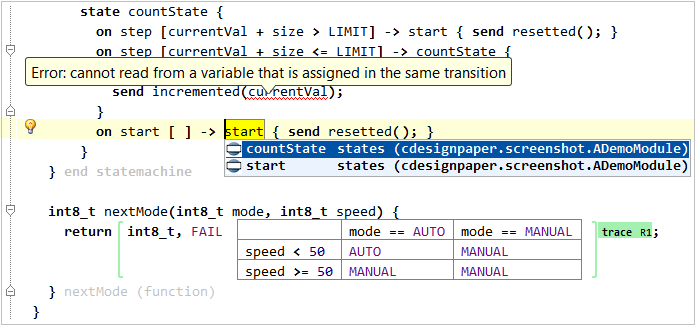
\includegraphics[width=8.6cm]{figures/screenshot.png}
\caption{An example of a program written with MPS. It mixed C functions,
state machines and decision tables, each of them defined as a separate
language. The screenshot also shows requirements traces (green annotations),
which can be attached to any program element without the definition of this
element being aware of the annotation.}
\label{screenshot}
\end{figure}

\section{Contents of the Tool Demo}

\pp{Introduction} We will introduce the need for language engineering in
the same way as in the introduction above. 

\pp{Example Use Case} We will then show an example from the mbeddr.com
extensible C language \cite{mbeddr}. The project develops modular extensions of
C to make embedded software development more productive. The project
demonstrates an intriguing use case fo language extension and showcases
syntactic forms other than text, such as the decision table shown in
\fig{screenshot}.

\pp{Creating Extensions} The main part of the demo will consist of a demo of how
to build a lanugage extension,


\section{What the audience will take away}



% For peer review papers, you can put extra information on the cover
% page as needed:
% \ifCLASSOPTIONpeerreview
% \begin{center} \bfseries EDICS Category: 3-BBND \end{center}
% \fi
%
% For peerreview papers, this IEEEtran command inserts a page break and
% creates the second title. It will be ignored for other modes.
\IEEEpeerreviewmaketitle




% conference papers do not normally have an appendix


% use section* for acknowledgement
\section*{Acknowledgment}


The authors would like to thank...
more thanks here


% trigger a \newpage just before the given reference
% number - used to balance the columns on the last page
% adjust value as needed - may need to be readjusted if
% the document is modified later
%\IEEEtriggeratref{8}
% The "triggered" command can be changed if desired:
%\IEEEtriggercmd{\enlargethispage{-5in}}

% references section

% can use a bibliography generated by BibTeX as a .bbl file
% BibTeX documentation can be easily obtained at:
% http://www.ctan.org/tex-archive/biblio/bibtex/contrib/doc/
% The IEEEtran BibTeX style support page is at:
% http://www.michaelshell.org/tex/ieeetran/bibtex/
%\bibliographystyle{IEEEtran}
% argument is your BibTeX string definitions and bibliography database(s)
%\bibliography{IEEEabrv,../bib/paper}
%
% <OR> manually copy in the resultant .bbl file
% set second argument of \begin to the number of references
% (used to reserve space for the reference number labels box)

% \nocite{*} 
\bibliographystyle{abbrv} 
\bibliography{tooldemo}






% that's all folks
\end{document}


